\chapter{Visualizing estimation results}
\label{visualization} \index{visualizing estimation results}

In this chapter we show, how estimation results produced with one of
the regression tools described in the two previous chapters can be
visualized. In general, there are two possibilities to visualize
results: Within {\em BayesX}, special functions can be applied to
regression objects. Since both regression tools provide almost the
same possibilities to visualize results, we describe them
simultaneously in the next section. Tools for the visualization of
autocorrelations for MCMC samples are described in
\autoref{plotautocor}. An alternative way to visualize results is to
use the S-Plus functions shipped together with BayesX. These
functions are described in \autoref{splus}.

\section{BayesX functions} \label{bayesxplot}

{\em BayesX} allows to visualize estimation results immediately
after estimation. The {\em output window} and/or the log file
describe how to do this for a particular model term. Nonlinear
effects of continuous covariates and time scales are plotted with
\hyperref[bayesxplotnonp]{method #plotnonp#}. Spatial effects are
visualized with \hyperref[drawmap]{method #drawmap#}. When using
{\em bayesreg objects}, autocorrelation functions of sampled
parameters can be visualized with \hyperref[plotautocor]{method
#plotautocor#}.

\newpage

\subsection{Method plotnonp} \label{bayesxplotnonp} \index{plotting
nonparametric functions} \index{plotnonp command}

\begin{stanza}{Description}

Method #plotnonp# is a post estimation command, i.e.~it is
meaningful only if method #regress# has been applied before. The
method allows to plot estimated effects of nonlinear covariate
effects immediately after estimation. T

\end{stanza}

\begin{stanza}{Syntax}

#># {\em objectname}.#plotnonp# {\em termnumber} [{\em , options}]


Plots the estimated effect with term number {\em termnumber}. The
term number will be printed in the {\em output window} and/or an
open log file. Several options are available for labelling axis,
adding a title, etc., see the options list below. Note that method
#plotnonp# can be applied only if random walks, P-splines or
seasonal components are used as priors.

\end{stanza}

\begin{stanza}{Options}

The following options are available for method #plotnonp# (listed
in alphabetical order):

\end{stanza}

\begin{itemize}
\item #connect=1#$|$#2#$|$#3#$|$#4#$|$#5#[{\em specifications for
further variables}]

Option #connect# specifies how points in the scatterplot are
connected. There are currently 5 different specifications:

\begin{tabular}{ll}
#1# & draw straight lines between the points (default) \\
#2#, #3#, #4# & draw dashed lines (numbers #2#-#4# indicate different variants)\\
#5# & do not connect, i.e.~plot points only \\
\end{tabular}

If you draw more than one scatterplot in the same graph (i.e. more
than one {\em yvar} is specified) you can connect points for every
{\em yvar} differently by simply specifying the corresponding
number (#1,2,3,4,5#) for every {\em yvar}. Typing for example

{\em #connect=15#}

connects the points corresponding to {\em yvar1} and {\em xvar} by
straight lines, but does not connect the points corresponding to
{\em yvar2} (if specified) and {\em xvar}. Points corresponding to
additionally specified variables $yvar3$, etc.~are connected by
straight lines.

An equivalent way of specifying the different variants is available
via the symbols #l#, #d#, #\_#, #-# and #p#, which correspond to the
numbers #1#-#5#, i.e.~

{\em #connect=12345#} is equivalent to {\em #connect=ld_-p#}

\item #fontsize = #{\em integer}

Specifies the font size (in pixels) for labelling axes etc. Note
that the title is scaled accordingly. The default is
#fontsize=12#.

\item #height = #{\em integer}

Specifies the height (in pixels) of the graph. The default is
#height=210#.

\item #levels = all#$|$#1#$|$#2#$|$#none#

By default, #plotnonp# plots the estimated nonlinear covariate
effect together with the pointwise credible intervals based on
nominal levels of 80\% and 95\% (the nominal levels may be changed
using the options \hyperref[level1]{level1} and/or
\hyperref[level2]{level2}). Option #levels# allows to omit
completely pointwise credible intervals in the graphs
(#levels=none#), print only the 95\% credible intervals
(#levels=1#) or to print only the 80\% credible intervals
(#levels=2#).

 \item #linecolor = B#$|$#b#$|$#c#$|$#G#$|$#g#$|$#o#$|$#m#$|$#r#$|$#y# [{\em specifications for further
variables}]

Option #linecolor# specifies the color to be used for drawing
lines (or points, see option #connect#) in the scatterplot.
Currently the following specifications are available:

\begin{tabular}{ll}
#B# & black (default) \\
#b# & blue \\
#c# & cyan \\
#G# & gray \\
#g# & green \\
#o# & orange \\
#m# & magenta \\
#r# & red \\
#y# & yellow
\end{tabular}

If you draw more than one scatterplot in the same graph (i.e. more
than one {\em yvar} is specified) you can use different colors for
each {\em yvar} by simply specifying the corresponding symbol
(#B,b,c,G,g,o,m,r,y#) for each {\em yvar}. Typing for example

{\em #linecolor = Bgr#}

colors the lines (points) corresponding to {\em yvar1} and {\em
xvar} in black, whereas the points corresponding to {\em yvar2}
and {\em yvar3} (if specified) and {\em xvar} are colored in green
and red, respectively.

\item #linewidth = #{\em integer}

Specifies how thick lines should be drawn. The default is
#linewidth=5#.

\item #outfile = #{\em characterstring}

If option #outfile# is specified the graph will be stored as a
postscript file rather than being printed on the screen. The path
and the filename must be specified in {\em characterstring}. By
default, an error will be raised if the specified file is already
existing or the specified folder is not existing. To overwrite  an
already existing file, option #replace# must be additionally
specified. This prevents you from unintentionally overwriting your
files.

\item #pointsize = #{\em integer}

Specifies the size of the points (in pixels) if drawing points
rather than lines is specified. The default is #pointsize=20#.

\item #replace#

The #replace# option is useful only in combination with option
#outfile#. Specifying #replace# as an additional option allows the
program to overwrite an already existing file (specified in
#outfile#), otherwise an error will be raised.

\item #title = #{\em characterstring}

Adds a title to the graph. If the title contains more than one
word, {\em characterstring} must be enclosed by quotation marks
(e.g. \texttt{title="my first title"}).

\item #titlesize = #{\em realvalue}

Specifies the factor by which the size of the title is scaled
relative to the size of the labels of the axes (compare option
#fontsize#). The default is \texttt{titlesize=1.5}.

\item #width = #{\em integer}

Specifies the width (in pixels) of the graph. The default is
#width=356#.

\item #xlab = #{\em characterstring}

Labels the x-axis. If the label contains more than one word, {\em
characterstring} must be enclosed by quotation marks (e.g.
\texttt{xlab="x axis"}).

\item #xlimbottom = #{\em realvalue}

Specifies the minimum value at the x-axis to be plotted. The
default is the minimum value in the data set. If #xlimbottom# is
above the minimum value in the data set, only a part of the graph
will be visible.

\item #xlimtop = #{\em realvalue}

Specifies the maximum value at the x-axis to be plotted. The
default is the maximum value in the data set. If #xlimtop# is
below the maximum value in the data set, only a part of the graph
will be visible.

\item #xstart = #{\em realvalue}

Specifies the value where the first 'tick' on the x-axis should be
drawn. The default is the minimum value on the x-axis.

\item #xstep = #{\em realvalue}

If #xstep# is specified,  ticks are drawn at the x-axis with
stepwidth {\em realvalue} starting at the minimum value on the
x-axis (or at the value specified in option #xstart#). By default,
five equally spaced ticks are drawn at the x-axis.

\item #ylab = #{\em characterstring}

Labels the y-axis. If the label contains more than one word, {\em
characterstring} must be enclosed by quotation marks (e.g.
\texttt{ylab="y axis"}).

\item #ylimbottom = #{\em realvalue}

Specifies the minimum value at the y-axis to be plotted. The
default is the minimum value in the data set. If #ylimbottom# is
above the minimum value in the data set, only a part of the graph
will be visible.

\item #ylimtop = #{\em realvalue}

Specifies the maximum value at the y-axis to be plotted. The
default is the maximum value in the data set. If #ylimtop# is
below the maximum value in the data set, only a part of the graph
will be visible.

\item #ystart = #{\em realvalue}

Specifies the value where the first 'tick' on the y-axis should be
drawn. The default is the minimum value on the y-axis.

\item #ystep = #{\em realvalue}

If #ystep# is specified,  ticks are drawn at the y-axis with
stepwidth {\em realvalue} starting at the minimum value on the
y-axis (or at the value specified in option #ystart#). By default,
five equally spaced ticks are drawn at the y-axis.
\end{itemize}

\newpage

\begin{stanza}{Examples}

Suppose we have already created a regression object #reg# and have
estimated a regression model with Gaussian errors using a command
like

#> reg.regress Y = X(psplinerw2), family=gaussian using d#

where #Y# is the response variable and #X# the only explanatory
variable. The effect of #X# is modelled nonparametrically using
Bayesian P-splines. In the {\em output window} we obtain the
following estimation output for the effect of #X#:

\begin{verbatim}
  f_x

  Results are stored in file
  c:\results\reg_f_x_pspline.res
  Results may be visualized using method plotnonp
  Type for example: objectname.plotnonp 0
\end{verbatim}

The term number of the effect of X is 0, i.e. by typing

#> reg.plotnonp 0#

we obtain the plot shown in \autoref{plotnonpexample1}.

Of course, a title, axis labels etc. can be added. For example by
typing

#> reg.plotnonp 0 , title="my title" xlab="x axis"#

we obtain the plot shown in \autoref{plotnonpexample2}.

By default, the plots appear in an additional window on the
screen. They can be directly stored in postscript format by adding
option #outfile#. For example by typing

 #> reg.plotnonp 0 , title="my title" xlab="x axis" outfile="c:\results\result1.ps"#

the graph is stored in postscript format in the file
#c:\results\result1.ps#.


\begin{figure}[p]
\begin{center}
\includegraphics[scale=0.8]{grafiken/plotnonpexample.ps}
{\em\caption{ \label{plotnonpexample1} Illustration for the usage of
method \em\tt plotnonp}}
\end{center}
\end{figure}


\begin{figure}[p]
\begin{center}
\includegraphics[scale=0.8]{grafiken/plotnonpexample2.ps}
{\em\caption{ \label{plotnonpexample2} Second illustration for the
usage of method \em\tt plotnonp}}
\end{center}
\end{figure}

\end{stanza}

\clearpage

\subsection{Method drawmap} \label{drawmap}
\index{drawmap command}

\begin{stanza}{Description}

Method #drawmap# is a post estimation command, i.e.~it is meaningful
only if method #regress# has been applied before. The method allows
to visualize estimated effects of spatial covariates immediately
after estimation.

\end{stanza}

\begin{stanza}{Syntax}

#># {\em objectname}.#drawmap# {\em termnumber} [{\em , options}]

Visualizes the effect of a spatial covariate by coloring the
regions of the corresponding geographical map according to the
estimated effect (or other characteristics of the posterior). The
term number {\em termnumber} identifies the model term and can be
found in the {\em output window} and/or an open log file. Several
options are available for adding a title or changing the color
scale etc., see the options list below. Note that method #drawmap#
can be applied only if Markov random fields, geosplines or
geokriging are used as priors.

\end{stanza}

\begin{stanza}{Options}

The following options are available for method #drawmap# (in
alphabetical order):

\end{stanza}

\begin{itemize}
\item #color#

The #color# option allows to choose between a grey scale for the
colors and a colored scale. If #color# is specified a colored
scale is used instead of a grey scale.

\item #drawnames#

In some situations it may be useful to print the names of the
regions into the graph (although the result may be confusing in
most cases). This can be done by specifying the additional option
#drawnames#. By default the names of the regions are omitted in
the map.

\item #lowerlimit = #{\em realvalue}

Lower limit of the range to be drawn. If #lowerlimit# is omitted,
the minimum numerical value in #plotvar# will be used instead as
the lower limit.

\item #nolegend#

By default a legend is drawn into the graph. By specifying the
option #nolegend# the legend will be omitted.

\item #nrcolors = #{\em integer}

To color the regions according to their numerical characteristics,
the data are divided into a (typically large) number of ordered
categories. Afterwards a color is associated with each category. The
#nrcolors# option can be used to specify the number of categories
(and with it the number of different colors). The maximum number of
colors is 256, which is also the default value.

\item #outfile = #{\em characterstring}

If option #outfile# is specified the graph will be stored as a
postscript file rather than being printed on the screen. The path
and the filename must be specified in {\em characterstring}. By
default, an error will be raised if the specified file is already
existing or the specified folder is not existing. To overwrite an
already existing file, option #replace# must be additionally
specified. This prevents you from unintentionally overwriting your
files.

\item #pcat#

If you want to visualize the values of the columns #pcat80# or
#pcat95# it is convenient to specify #pcat#. This forces #drawmap#
to expect a column that consists only of the values -1, 0 and 1. Of
course you can achieve the same result by setting #nrcolors=3#,
#lowerlimit=-1# and #upperlimit=1#.

\item #plotvar = #{\em variablename}

By default, the regions of the map are colored according to the
estimated spatial effect. Option #plotvar# allows to color the map
according to other characteristics of the posterior by explicitly
specifying the name of the variable to be plotted. Compare the
header of the file containing the estimation results to see all
variables available for plotting.

\item #replace#

The #replace# option is only useful in combination with option
#outfile#. Specifying #replace# as an additional option allows the
program to overwrite an already existing file (specified in
#outfile#), otherwise an error will be raised.

\item #swapcolors#

In some situations it may be favorable to swap the order of the
colors, i.e.~black (red) shades corresponding to large values and
white (green) shades corresponding to small values. This is
achieved by specifying #swapcolors#. By default, small values are
colored in black shades (red shades) and large values in white
shades (green shades).

\item #title = #{\em characterstring}

Adds a title to the graph. If the title contains more than one
word, {\em characterstring} must be enclosed by quotation marks
(e.g. #title="my first map"#).

\item #upperlimit = #{\em realvalue}

Upper limit of the range to be plotted. If #upperlimit# is
omitted, the maximum numerical value in #plotvar# will be used
instead as the upper limit.

\end{itemize}


\begin{stanza}{Examples}

Suppose we have already created a regression object #reg# and have
estimated a regression model with Gaussian errors using something
like

#> map m# \\
#> m.infile using c:\maps\map1.bnd#

#> reg.regress Y = region(spatial,map=m), family=gaussian using d#

where #Y# is the response variable and #region# the only
explanatory variable. The effect of the spatial covariate #region#
is modelled nonparametrically  using a Markov random field. In the
{\em output window} we obtain the following estimation output for
the effect of #region#:

\begin{verbatim}
  f_spat_region

  Results are stored in file
  c:\results\reg_f_region_spatial.res
  Results may be visualized using method 'drawmap'
  Type for example: objectname.drawmap 0
\end{verbatim}

The term number of the effect of #region# is 0, i.e.~by typing

#> reg.drawmap 0#

we obtain the map shown in \autoref{drawmapexample1} where the
regions are colored according to the estimated spatial effect.

By default the regions are colored in grey scale. A color scale is
obtained by adding option #color#. A title can be added as well.
For example by typing

#> reg.drawmap 0 , color title="my title"#

we obtain the map shown in \autoref{drawmapexample2}.

By default, the maps appear in an additional window on the screen.
They can be directly stored in postscript format by adding option
#outfile#. For example by typing

 #> reg.drawmap 0 , color title="my title" outfile="c:\results\result1.ps"#

the colored map is stored in postscript format in the file
#c:\results\result1.ps#.

\begin{figure}[ht]
\begin{center}
\includegraphics[scale=0.4]{grafiken/drawmapexample.ps}
{\em\caption{ \label{drawmapexample1} Illustration for the usage
of method \em \texttt{drawmap}}}
\end{center}
\end{figure}


\begin{figure}[ht]
\begin{center}
\includegraphics[scale=0.4]{grafiken/drawmapexample2.ps}
{\em\caption{ \label{drawmapexample2} Second illustration for the
usage of method \em \texttt{drawmap}}}
\end{center}
\end{figure}

\end{stanza}

\clearpage

\subsection{Method plotautocor} \label{plotautocor}
\index{plotautocor command}

\begin{stanza}{Description}

Method #plotautocor# is a post estimation command, i.e.~it is
meaningful only if method #regress# has been applied before.
Method #plotautocor# computes and visualizes the autocorrelation
functions of the parameters in the model. This method is only
applicable to {\em bayesreg objects}.

\end{stanza}

\begin{stanza}{Syntax}

#># {\em objectname}.#plotautocor# [{\em , options}]

Computes and visualizes the autocorrelation functions in the
model. Several options are available for specifying the maximum
lag for autocorrelations, storing the graphs in postscript format
etc., see the options list below.

\end{stanza}

\begin{stanza}{Options}

The following options are available for method #plotautocor# (in
alphabetical order):

\end{stanza}

\begin{itemize}
\item #maxlag = #{\em integer}

Option #maxlag# may be used to specify the maximum lag for
autocorrelations. The default is #maxlag=250#.

\item #mean#

If option #mean# is specified, for each lag number and model term
only minimum, mean and maximum autocorrelations are plotted. This
can lead to a considerable reduction in computing time and storing
size.

\item #outfile = #{\em characterstring}

If option #outfile# is specified the graph will be stored as a
postscript file and not printed on the screen. The path and the
filename must be specified in {\em characterstring}. An error will
be raised if the specified file is already existing and the
#replace# option is not specified.

\item #replace#

The #replace# option is only useful in combination with option
#outfile#. Specifying #replace# as an additional option allows the
program to overwrite an already existing file (specified in
#outfile#), otherwise an error will be raised.
\end{itemize}

\begin{stanza}{Examples}

Suppose we have already created a {\em bayesreg object} #reg# and
have estimated a regression model with Gaussian errors using

#> reg.regress Y = X(psplinerw2), family=gaussian using d#

where #Y# is the response variable and #X# the only explanatory
variable. The effect of #X# is modelled nonparametrically  using
Bayesian P-splines. We can now check the mixing of sampled
parameters by computing and drawing the autocorrelation functions
up to a maximum lag of 150:

#> reg.plotautocor , maxlag=150 outfile="c:\results\autocor.ps"#

In this example the autocorrelation functions are not shown on the
screen but stored in postscript format in the file
#c:\results\autocor.ps#. If option #outfile# is omitted, the
functions are plotted on the screen. The resulting file contains 5
pages. As an example, the first page of the file is shown in
\autoref{autocorexample}.

\begin{figure}[ht]
\begin{center}
\includegraphics[scale=0.8]{grafiken/autocorexample1.ps}
{\em\caption{ \label{autocorexample} Illustration for the usage of
method \em\texttt{plotautocor}}}
\end{center}
\end{figure}

\end{stanza}

\clearpage

\section{S-plus functions} \label{splus} \index{S-plus functions}

Some S-plus and R functions for plotting estimated functions are
shipped together with {\em BayesX}. These functions can be found in
the subdirectory #sfunctions# of the installation directory.
\autoref{plotfunctions} gives a first overview over the different
functions and their abilities. The usage of the functions is very
simple so that also users not familiar with the S-plus environment
should be able to apply the functions without any difficulties. The
following subsections describe how to install the functions in
S-plus and give a detailed description of the usage of the
respective functions.

\begin{table}[ht]
\begin{center}
\begin{tabular}{|l|l|}
\hline
{\bf Functionname} & {\bf Description} \\
\hline
#plotnonp# & visualizes estimated nonparametric functions \\
#plotautocor# & visualizes autocorrelation functions \\
#plotsample# & visualizes sampling paths of sampled parameters \\
#readbndfile# & reads in boundaries of geographical maps \\
#drawmap# & visualizes estimation results for spatial covariates \\
#plotsurf# & visualizes estimated 2 dimensional surfaces \\
\hline
\end{tabular}
{\em\caption{\label{plotfunctions} Overview over S-plus
functions}}
\end{center}
\end{table}


\subsection{Installation of the functions} \index{S-plus
functions!installation}

Installation of the different functions is very easy. The S-plus
code for the functions is stored in the directory {\em
$<$INSTALLDIRECTORY$>$}#\sfunctions# in the ASCII text file
#plot.s#. To install the functions you first have to start S-plus.
Afterwards the functions will be installed by entering

#> source("#{\em $<$INSTALLDIRECTORY$>$}#\\sfunctions\\plot.s")#

in the {\em Commands Window} of S-plus. Note that a double backslash
is required in S-plus to specify a directory correctly. For use with
the R package the file #plot.r# is supplied, which contains slightly
modified versions of the S-plus functions.

\subsection{Plotting nonparametric functions} \label{splusplotnonp}
\index{S-plus functions!plotting nonparametric functions}
\index{plotting nonparametric functions}

This subsection describes the usage of the function #plotnonp# for
visualizing nonparametric function estimates.

Suppose that a Bayesian regression model has already been
estimated with predictor

$$
\eta = \dots + f(X) + \dots,
$$

where the effect of #X# is modelled nonparametrically using for
example a first or second order random walk prior. Unless the
directory for estimation output has been changed using the global
option #outfile# (see \autoref{bayesregglobopt} and
\autoref{remlregglobopt}), estimation results for the
nonparametric effect of #X# are stored in the directory

{\em$<$INSTALLDIRECTORY$>$}#\output#

that is in the subdirectory #output# of the installation
directory. The filename is

{\em objectname}#_f_X_rw.res#

that is it is composed of the name of the regression object and
the covariate name. For the following we assume that #c:\bayes# is
the installation directory and #reg# is the name of the regression
object. In this case results for the effect of #X# are stored in:

#c:\bayes\output\reg_f_X_rw.res#

The structure of such a file has already been described in
\autoref{bayesregress} ({\em bayesreg objects}) and
\autoref{remlregregress} ({\em remlreg objects}). Although it is
possible (and very easy) to visualize the estimated nonparametric
function with any software package that has plotting capabilities, a
fast and easy way of plotting estimation results without knowing the
particular structure of the results-file is desirable. This is the
task of the S-plus function #plotnonp#.

The function has only one required and many optional arguments.
The required argument is the directory and the filename where
nonparametric estimation results are stored. For example by
entering the command

#> plotnonp("c:\\bayes\\output\\reg_f_X_rw.res")#

a S-plus {\em graphic window} will be opened with the plotted
function estimate. The function plots the estimated effect
together with the posterior 2.5\%, 10\%, 90\% and 97.5\%
quantiles. One advantage of the function is that after its
application no permanent objects will remain in the S-plus
environment.

Besides the required argument a lot of optional arguments may be
passed to the function. Among others there are options for
plotting the graphs in a postscript file rather than the screen,
labelling the axes, specifying the minimum/maximum value on the
x/y axes and so on. The following optional arguments can be passed
to #plotnonp#:

\begin{itemize}
\item #psname = "#{\em filename (including path)}#"#\\
Name of the postscript output file. If #psname# is specified the
graph will be stored in a postscript file and will not appear on
the screen.

\item #level = 0#|#1#|#2# \\
Specifies whether to plot only the 95\% credible intervals
(#level=1#) or only the 80\% credible intervals (#level=2#).
Default value is #level=0#, i.e.~both.

\item #ylimtop = #{\em realvalue} \\
Specifies the maximum value on the y-axis (vertical axis).

\item #ylimbottom = #{\em realvalue}\\
Specifies the minimum value on the y-axis.

\item #xlab = "#{\em characterstring}#"# \\
#xlab# is used to label the x-axis (horizontal axis).

\item #ylab = "#{\em characterstring}#"# \\
#ylab# is used to label the y-axis.

\item #maintitle = "#{\em characterstring}#"# \\
Adds a title to the graph.

\item #subtitle = "#{\em characterstring}#"# \\
Adds a subtitle to the graph.

\item #linecol = #{\em integer} \\
Specifies the color of the credible intervals. Default value is
#linecol=3#.

\item #linetype = #{\em integer} \\
Specifies the line type for the credible intervals. Default value
is #linetype=1# (solid).
\end{itemize}

As an illustration compare the following S-plus statement:

#> plotnonp("c:\\bayes\\reg_f_X_rw.res", psname="c:\\bayes\\reg_f_X_rw.ps", #\\
#  maintitle="Maintitle",ylab="effect of X",xlab="X") #

\begin{figure}[ht]
\begin{center}
%\includegraphics[scale=0.8]{b_nonpX.eps}
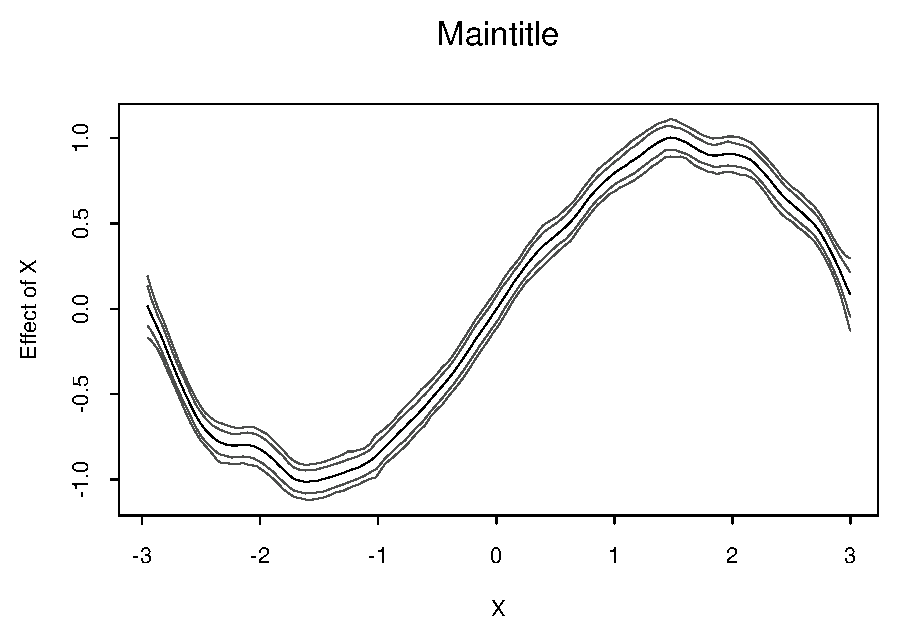
\includegraphics[scale=0.8]{grafiken/plotnonp.eps}
{\em\caption{ \label{illgraph} Illustration for the usage of
\em\tt plotnonp}}
\end{center}
\end{figure}

This statement draws the estimated effect of #X# and stores the
graph in the postscript file #"c:\\bayes\\reg_f_X_rw.ps"#. A
title, a x-axis and y-axis label are added to the graph. For
illustration purposes, the resulting graph is shown in
\autoref{illgraph}.

In some situations the effect of a covariate representing dates
must be plotted. Suppose for example that a covariate has values
ranging from 1 to 19 representing the time period from January
1983 to July 1984. In this case, we naturally prefer that the
x-axis is labelled in terms of dates rather than in the original
coding (from 1 to 19). To achieve this, function #plotnonp#
provides the three additional options #year#, #month# and #step#.
Options #year# and #month# are used to specify the year and the
month (1 for January, 2 for February, \dots) corresponding to the
minimum covariate value. In the example mentioned above
#year=1983# and #month=1# will produce the correct result. In
addition, option #step# may be specified to define the periodicity
in which your data are collected. For example #step=12# (the
default) corresponds to monthly data, while #step=4#, #step=2# and
#step=1# correspond to quarterly, half yearly and yearly data. We
illustrate the usage of #year#, #month# and #step# with our
example. Suppose we estimated the effect of calendar time #D#,
say, on a certain dependent variable, where the range of the data
is as described above. Then the following S-plus function call
will produce the postscript file shown in \autoref{illgraph2}:

\begin{figure}[ht]
\begin{center}
%\includegraphics[scale=0.8]{fvdate.eps}
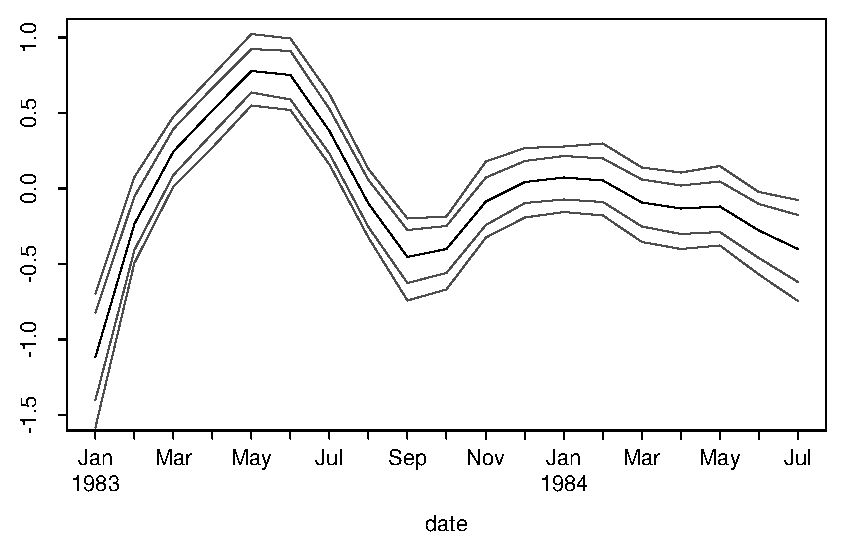
\includegraphics[scale=0.8]{grafiken/plotnonpdate.eps}
{\em\caption{ \label{illgraph2} Illustration for the usage of
\em\tt plotnonp}}
\end{center}
\end{figure}

#> plotnonp("c:\\bayes\\reg_f_D_pspline.res",psname="c:\\bayes\\reg_f_D_pspline.ps",#\\
#  year=1983,month=1,step=12,xlab="date",ylab= " ") #

Note, that \texttt{ylab=" "} forces S-plus to omit the y-axis label.
If #ylab# (as well as #xlab#) is omitted, default labels will be
given to the two axis.

Finally, we note that all options that can be passed to the #plot#
function of S-plus may also be passed to function #plotnonp#.
Thus, function #plotnonp# is more or less a specialized version of
the S-plus #plot# function.


\subsection{Drawing geographical maps} \index{S-plus!drawing
geographical maps} \index{drawing geographical maps}

This subsection describes how to visualize estimation results of
spatial covariates, where the observations represent the location
or site in connected geographical regions. A typical example for a
spatial covariate is given in the 'rents for flats' example, see
\autoref{rentdata}, where the covariate #L# indicates the location
(in subquarters) of the flat in Munich. \autoref{munich} shows a
map of Munich separated into subquarters.

\begin{figure}
\centering
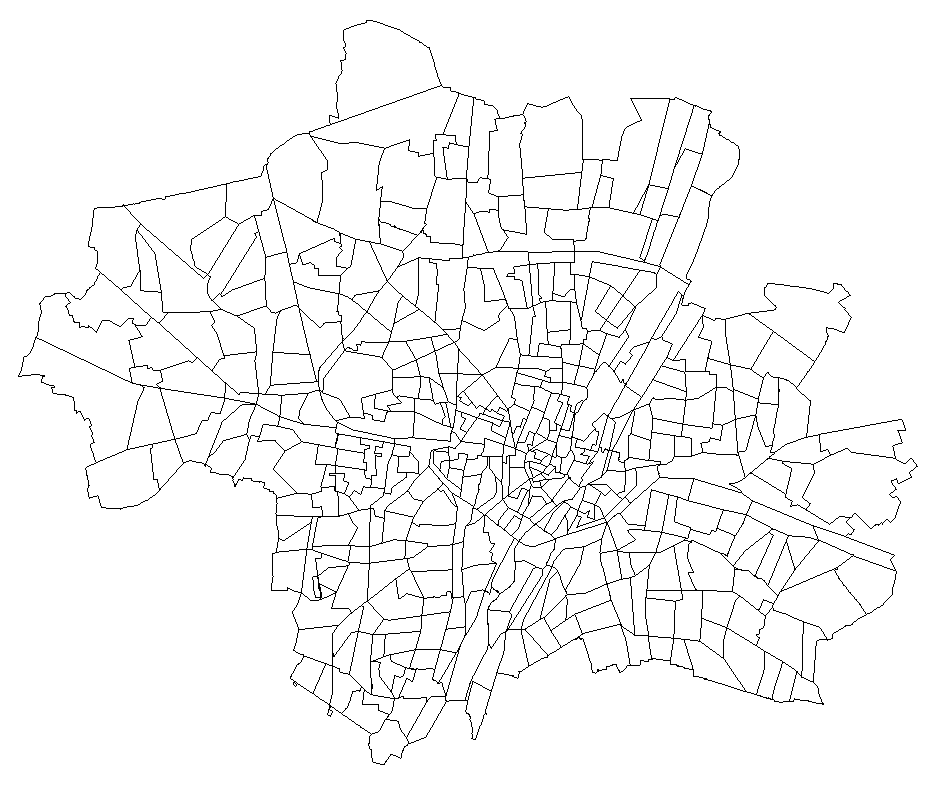
\includegraphics [scale=0.5]{grafiken/munich.eps}
{\em\caption{\label{munich} Map of Munich}}
\end{figure}


Typically, the effect of such a spatial covariate is incorporated
into a regression model via an unstructured or structured random
effect. In the latter case a spatial smoothness prior for the
spatial covariate is specified that penalizes too abrupt changes of
the estimated effect in neighboring sites. In some situations the
incorporation of both, an unstructured and a structured effect, may
also be appropriate. Details on how to incorporate spatial
covariates into a semiparametric regression  model are given in
\autoref{bayesregress} ({\em bayesreg objects}) and
\autoref{remlregregress} ({\em remlreg objects}). For the rest of
this section we assume that an effect of a spatial covariate has
already been estimated and that we now want to visualize the
estimation results. This can be easily done with the two S-plus
functions #readbndfile# and #drawmap#. Function #readbndfile# is
used to read the boundary information of a map that is stored in a
so called boundary file and to store this information as a permanent
S-plus {\em map object}. The boundary file contains mainly the
polygons which form the different geographical regions of the map.
The required structure of such a file is described below. After the
successful reading of the boundary information of a map, the second
function #drawmap# may be used to draw and print the map either on
the screen or into a postscript file. There are several possible
ways to draw the map. In the simplest case the map can be drawn
without any estimation effects, i.e.~only the boundaries of the
different regions or sites are drawn, see \autoref{munich} for an
example. In practice, however, one usually wants to color the
regions of the map according to some numerical characteristics. As
an example compare \autoref{munichrelfreq} in which the subquarters
of Munich are colored according to the frequency of flats in the
'rents for flats' data set located in the respective subquarter.
Subquarters colored in red contain less flats compared to
subquarters colored in green. In striped areas no observations are
available.

\begin{figure}[ht]
\begin{center}
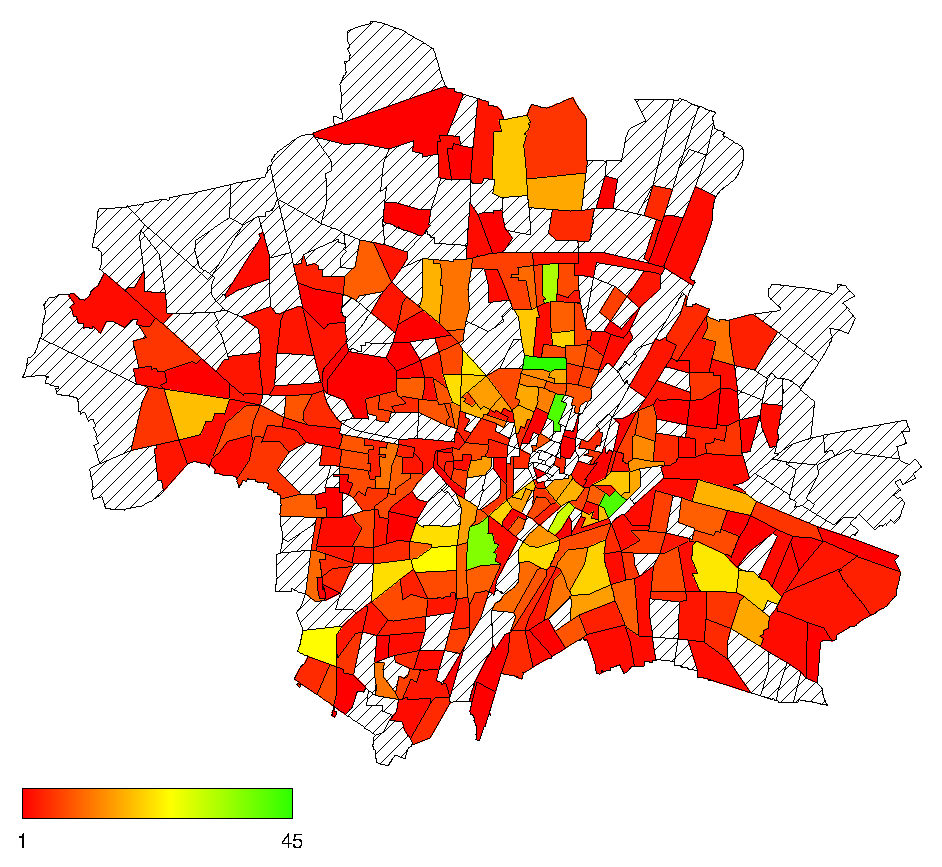
\includegraphics[scale=0.5]{grafiken/munichfr.eps}
{\em\caption{ \label{munichrelfreq} relative frequencies of
observed flats in the 'rents for flats' data set}}
\end{center}
\end{figure}


In the following we give a detailed description of the usage of
the functions #readbndfile# and #drawmap#.

\subsubsection*{Function readbndfile}
\index{S-plus!reading boundary files} \index{reading boundary
files}

Function #readbndfile# is used to read in boundary information
stored in a boundary file into S-plus. The function has two
required arguments. The first argument is the filename of the
boundary file to read in. The second argument specifies the name
of the {\em map object} in S-plus (recall that the map information
is stored as a permanent S-plus object). To give an example,
suppose that {\em BayesX} is installed in the directory #c:\bayes#
and that we want to read in the map of Munich. In this case the
boundary file of the map is stored in the subdirectory #examples#
of the installation directory, that is in #c:\bayes\examples#. The
name of the boundary file is simply #munich.bnd#. The following
function call reads in the boundary information of Munich and
stores the map permanently in S-plus:

#> readbndfile("c:\\bayes\\examples\\munich.bnd","munich")#

Once again, note that double backslashes are required in S-plus to
specify a directory. The second argument in the statement above is
"munich", i.e.~the name of the map object is simply #munich#. To
refer to the map of Munich in subsequent statements and function
calls, the quotation marks must be omitted.

\subsubsection*{Function drawmap}
\index{S-plus!drawmap}

Function #drawmap# is used to draw geographical maps and color the
regions according to some numerical characteristics. There is only
one required argument that must be passed to #drawmap#, that is
the name of the map to be drawn. Provided that the map has already
been read into S-plus (via function #readbndfile#), the following
statement draws the map of Munich in a S-plus graphic-window on
the screen:

#> drawmap(map=munich)#

Storing the map in a postscript file rather than drawing it on the
screen can be achieved by specifying the name of the postscript
file using the #outfile# option. For example the command

#> drawmap(map=munich,outfile="c:\\bayes\\munich.ps")#

produces a postscript file named #munich.ps# with the map of
Munich.

However, in most cases one not only wants to draw the boundaries of
a geographical map, but also color the regions according to some
numerical characteristics. Suppose for example that we have already
estimated a location specific effect on the monthly rents in the
'rents for flats' data set. Suppose further that the estimated
effects are stored in #c:\bayes\output\reg_f_L_spatial.res#. The
structure of the file is described in detail in
\autoref{bayesregress} ({\em bayesreg objects}) and
\autoref{remlregregress} ({\em remlreg objects}).

Suppose now that we want to visualize estimation results for the
spatial covariate #L# by coloring the subquarters of Munich
according to the posterior mean estimated using a {\em bayesreg
object}. Compared to the S-plus statement above, (at least) three
more arguments must be passed to function #drawmap#; the argument
#dfile# that specifies the filename of estimated results, the
argument #plotvar# that specifies the variable to be plotted and
the argument #regionvar# that specifies which column of the file,
containing estimation results, stores the region names. The
following statement produces the desired result:

 #> drawmap(map=munich,outfile="c:\\bayes\\munich.ps", #\\
 #  dfile="c:\\bayes\\output\\reg_f_L_spatial.res", plotvar="pmean",regionvar="L")#

Note that the right hand side of options #plotvar# and #regionvar#
must be enclosed by quotation marks. If we want to color the
subquarters of Munich according to the posterior mode estimated
using a {\em remlreg object} we have to change the statement to

 #> drawmap(map=munich,outfile="c:\\bayes\\munich.ps", #\\
 #  dfile="c:\\bayes\\output\\reg_f_L_spatial.res", plotvar="pmode",regionvar="L")#

\subsubsection*{Optional arguments of function drawmap}

Besides the arguments discussed so far there are some more
optional arguments that can be passed to #drawmap#. They are
listed and described below together with a summary of the
arguments already described:


\begin{itemize}
\item #map = "#{\em characterstring}#"#

Name of the S-plus {\em map object}. Use function #readbndfile# to
read in geographical maps into S-plus.

\item #dfile = "#{\em filename (including path)}#"#

Filename (including path) of the file containing numerical
characteristics of the regions of the map. The file must contain
at least two columns, one column that lists the names of the
regions and one column containing the numerical characteristics of
the respective regions. It is important that the names of the
regions listed match with the region names stored in the S-plus
{\em map object}. The first row of the file must contain the names
of the columns.

\item #outfile = "#{\em filename (including path)}#"#

Filename (including path) of the postscript file where the map
should be stored.

\item #regionvar = "#{\em characterstring}#"#

Name of the column in the data file containing the region names
(see also argument #dfile#). Note that the right hand side must be
enclosed by quotation marks.

\item #plotvar = "#{\em characterstring}#"#

Name of the column in the data file containing the numerical
characteristics of the regions (see also argument #dfile#). Note
that the right hand side must be enclosed by quotation marks.

\item #lowerlimit = #{\em realvalue}

Lower limit of the range to be drawn. If #lowerlimit# is omitted,
the minimum numerical value in the #plotvar# column will be used
instead as the lower limit.

\item #upperlimit = #{\em realvalue}

Upper limit of the range to be drawn. If #upperlimit# is omitted,
the maximum numerical value in the #plotvar# column will be used
instead as the upper limit.

\item #nrcolors = #{\em integer}

To color the regions according to their numerical characteristics,
the data are divided into a (typically large) number of ordered
categories. Afterwards a color is associated with each category.
The #nrcolors# option can be used to specify the number of
categories (and with it the number of different colors). Default
value is 100.

\item #pstitle = "#{\em characterstring}#"#

Adds a title to the graph. Note that the right hand side must be
enclosed by quotation marks.

\item #color = T#/#F#

The #color# option allows to choose between a grey scale for the
colors and a colored scale. The default is #color=F#, which means
a grey scale.

\item #legend = T#/#F#

By default a legend is drawn into the graph. To omit the legend in
the graph, #legend=F# must be passed as an additional argument.

\item #drawnames = T#/#F#

In some situations it may be favorable to print the names of the
regions into the graph (although the result may be confusing in
most cases). This can be done by specifying the additional option
#drawnames=T#. By default the names of the regions are omitted in
the graph.

\item #swapcolors = T#/#F#

In some situations it may be favorable to swap the order of the
colors, i.e.~red shades corresponding to large values and green
shades corresponding to small values. This is achieved by
specifying #swapcolors=T#. By default small values are colored in
red shades and large values in green shades.

\item #pcat = T#/#F#

If you want to visualize the values of the columns #pcat80# or
#pcat95# it is convenient to specify #pcat=T#. This forces
#drawmap# to expect a column that consists only of the values -1,
0 and 1. Of course you can achieve the same result by setting
#nrcolors=3#, #lowerlimit=-1# and #upperlimit=1#. The default is
#pcat=F#.
\end{itemize}

\subsection{Plotting 2 dimensional surfaces}
\label{splusplotsurf} \index{S-plus!plotting 2 dimensional surfaces}
\index{plotting 2 dimensional surfaces}

This subsection describes the usage of the function #plotsurf# for
visualizing 2 dimensional surfaces. The function #plotsurf# merely
invokes different S-plus functions for visualizing 2 dimensional
data. Thus, users familiar with S-plus may prefer to use this
functions directly to gain more flexibility. Note that this
function is only available for S-plus and not for R.

Suppose that a Bayesian regression model has already been
estimated with predictor

$$
\eta = \dots + f(X1,X2) + \dots,
$$

where the interaction effect of #X1# and #X2# is modelled
nonparametrically using 2 dimensional P-splines and that the
estimation results are stored in file:

#c:\bayes\output\reg_f_X1_X2_pspline.res#

The S-plus function #plotsurf# requires at least one argument,
which is the name (including path) of the file containing the
estimation results. For example the command

#> plotsurf("c:\\bayes\\output\\reg_f_X1_X2_pspline.res")#

plots the estimated surface against #X1# and #X2# on the screen.
There are several additional options that can be passed, for
example for changing the plot type or storing the graph as a
postscript file rather than displaying it on the screen. The
following list describes all possible arguments that may be passed
to the function #plotsurf#:

\begin{itemize}
\item #data = "#{\em filename (including path)}#"#

Name (including path) of the file containing the estimation
results. The file must contain at least 3 columns, one for the
x-axis, one for the y-axis and one for the z-axis. The file must
contain a header.

\item #outfile = "#{\em filename (including path)}#"#

Name (including path) of the postscript file where the graph
should be stored. This option is only meaningful for #mode=2# and
#mode=3#.

\item #cols = #{\em 3 column vector}

This option is only meaningful, if the argument #data# is
specified. In this case #cols# gives the columns of the object or
data file passed to the argument #data#, that should be used as
values for the x, y and z axis. The default is #cols=c(2,3,4)#
which corresponds to plotting the estimated surface against #X1#
and #X2#.

%\item {\bf zlim = 2 column vector}

%2 column vector giving the minimum and maximum value to be put on
%the z-axis.

\item #mode = 1#/#2#/#3#/#4#/#5#

This option specifies the plot type. Currently there are 5
different types available. The default is #mode=1#, which
corresponds to what is called a 'Surface Plot' in S-plus.
\end{itemize}

\subsection{Plotting autocorrelation functions}
\label{splusplotautocor} \index{S-plus!plotting autocorrelation
functions} \index{plotting autocorrelation functions}
\index{autocorrelation functions!plotting}

This section describes how to visualize autocorrelation functions
of sampled parameters using the S-plus function #plotautocor#.

To compute autocorrelation functions, the post-estimation command
#autocor# must be applied, see \autoref{bayesautocorr} for
details. For the rest of this section we assume that
autocorrelations are already computed and stored in file:

#c:\bayes\output\reg_autocor.raw#

The minimum number of arguments required for the function is one,
namely the file where the computed autocorrelation functions are
stored. In this case a S-plus {\em graphic window} will be opened
and the autocorrelation functions are plotted on the screen. To
store autocorrelations in a postscript file, an output filename
must be specified as a second argument. Thus, the S-plus command

#> plotautocor("c:\\bayes\\output\\reg_autocor.raw")#

prints autocorrelations on the screen, while the statement

 #> plotautocor("c:\\bayes\\output\\reg_autocor.raw","c:\\bayes\\output\\reg_autocor.ps")#

forces S-plus to store the autocorrelation graphs in the
postscript file #c:\bayes\output\reg_autocor.ps#.

In particular for regression models with a large number of
parameters the execution of function #plotautocor# can be very time
consuming. Moreover, the size of the resulting postscript file can
be very large. To avoid such problems #plotautocor# provides the
additional argument #mean.autocor#. If #mean.autocor=T# is
specified, for each lag number and model term only minimum, mean and
maximum autocorrelations are plotted, leading in most cases to a
considerable reduction in computing time and storing size.

\subsection{Plotting sampled parameters} \label{splusplotsample}
\index{S-plus!plotting sampled parameters} \index{plotting sampled
parameters}

This section describes how to plot sampled parameters using the
S-plus function #plotsample#. Before applying function
#plotsample#, sampled parameters must be stored in ASCII-format
using the post-estimation command #getsample#. See
\autoref{bayesgetsample} for details, but note that sampled
parameters will be stored in several different files, typically
one file for each term in the model.

Suppose now that we want to visualize sampling paths for the
parameters of the nonlinear effect of a covariate X. Assume
further that sampled parameters are stored in the ASCII file

#c:\bayes\output\reg_X_sample.raw#.

As most other functions, #plotsample# provides two possibilities
of drawing sampled parameters. The first possibility is to print
the graphs on the screen, and the second is to store them into a
postscript file. To print the sampling paths on the screen, only
the filename (including path) of the ASCII file where sampled
parameters are stored must be passed to the function. For the
example mentioned above the corresponding command is:

#> plotsample("c:\\bayes\\output\\reg_X_sample.raw")#

If sampling paths should be drawn into a postscript file rather
than on the screen, the filename of the resulting postscript file
must be specified as a second argument. Thus, for our example we
get:

 #> plotsample("c:\\bayes\\output\\reg_X_sample.raw","c:\\bayes\\output\\reg_X_sample.ps")#

In addition, all options that are available for the S-plus
function #plot# may be passed to function #plotsample#, see the
S-plus documentation for details.
